\documentclass[aspectratio=169,11pt]{beamer}

\usepackage{graphicx}
\usepackage{tikz}
\usetikzlibrary{positioning,arrows.meta}
\usepackage{xcolor}
\usepackage{booktabs}
\usepackage{tabularx}
\usepackage{array}
\usepackage{ragged2e}

\definecolor{GEUBlue}{RGB}{20,55,105}
\definecolor{GEULightBlue}{RGB}{238,244,251}
\definecolor{GEUGrey}{RGB}{90,90,90}
\definecolor{GEULightGrey}{RGB}{245,246,248}

\usetheme{default}
\setbeamertemplate{navigation symbols}{}
\setbeamertemplate{blocks}[rounded][shadow=false]
\setbeamercolor{normal text}{fg=black,bg=white}
\setbeamercolor{frametitle}{fg=GEUBlue}
\setbeamercolor{structure}{fg=GEUBlue}
\setbeamercolor{block title}{fg=GEUBlue,bg=GEULightBlue}
\setbeamercolor{block body}{fg=black,bg=GEULightBlue}
\setbeamerfont{frametitle}{size=\Large,series=\bfseries}

% Replace with the actual logo filename
\newcommand{\GEULogo}{graphicera_logo.png}

% Header and footer
\setbeamertemplate{headline}{%
  \begin{tikzpicture}[remember picture,overlay]
    \node[anchor=north east,xshift=-0.30cm,yshift=-0.12cm]
      at (current page.north east)
      {\includegraphics[height=0.62cm]{\GEULogo}};
  \end{tikzpicture}
  \vspace{0.72cm}
}
\setbeamertemplate{frametitle}{%
  \vspace{0.03cm}
  \insertframetitle\par
  \vspace{0.04cm}
  \textcolor{GEUBlue}{\rule{\textwidth}{0.9pt}}
  \vspace{0.03cm}
}
\setbeamertemplate{footline}{%
  \leavevmode
  \hbox{%
  \begin{beamercolorbox}[wd=.82\paperwidth,ht=0.32cm,dp=0.10cm,leftskip=.3cm]{author in head/foot}
    \tiny Department of Computer Science \& Engineering | Graphic Era (Deemed to be University)
  \end{beamercolorbox}%
  \begin{beamercolorbox}[wd=.18\paperwidth,ht=0.32cm,dp=0.10cm,rightskip=.3cm]{date in head/foot}
    \hfill\tiny\insertframenumber/\inserttotalframenumber
  \end{beamercolorbox}}
}

\newcommand{\smallnote}[1]{\vspace{0.08cm}{\scriptsize\color{GEUGrey}#1}}
\newcommand{\placeholder}[1]{\textit{\color{GEUGrey}#1}}

\title{\textbf{Project-Based Learning}\\[2mm]\large Phase-I Evaluation}
\author{\textbf{Project Title}\\Team ID: XXXX}
\institute{Department of Computer Science \& Engineering\\Graphic Era (Deemed to be University), Dehradun}
\date{Academic Session 2026--27}

\begin{document}

% 1
\begin{frame}[plain]
\begin{tikzpicture}[remember picture,overlay]
\draw[GEUBlue,line width=3pt] (current page.north west) -- (current page.north east);
\node[anchor=north east,xshift=-0.45cm,yshift=-0.35cm] at (current page.north east)
{\includegraphics[height=1.0cm]{\GEULogo}};
\node[align=center,text width=.84\paperwidth] at ([yshift=.25cm]current page.center)
{{\color{GEUBlue}\fontsize{26}{30}\selectfont\bfseries PROJECT-BASED LEARNING}\\[3mm]
 {\fontsize{18}{22}\selectfont PHASE-I EVALUATION}\\[7mm]
{\color{GEUGrey}\Large\bfseries
ScamShield: Explainable Multimodal AI for Intelligent Scam and Phishing Detection\\
For Reducing Cyber Crime Risks}
 \\
 \vspace{2mm}

 {\color{GEUBlue}\normalsize Team ID: DSCPP-III-2026-T122}};
\node[align=center,anchor=south,yshift=.42cm] at (current page.south)
{\bfseries Department of Computer Science \& Engineering\\
Graphic Era (Deemed to be University), Dehradun\\[-1mm]
\scriptsize Academic Session 2026--27};
\end{tikzpicture}
\end{frame}

% 2
\begin{frame}{Team \& Mentor Details}
\begin{columns}[T,totalwidth=\textwidth]
\column{.48\textwidth}
\begin{block}{Team Information}
\begin{tabular}{@{}ll@{}}
\textbf{Team ID:} & DSCPP-III-2026-T122\\
\textbf{Semester:} & 3rd \\
\textbf{Section:} & ML2,ML3,DS1\\
\textbf{Domain:} & \placeholder{Cybersecurity + AI/ML}
\end{tabular}
\end{block}
\column{.48\textwidth}
\begin{block}{Team Members}
1.\quad \placeholder{Shivansh Bajaj -- 2510370470}\\
2.\quad \placeholder{Ashrey Goel -- 2510370302}\\
3.\quad \placeholder{Kangana Agarwal -- 2510380099}\\
\end{block}
\end{columns}
\vspace{2mm}
\begin{block}{Mentor}
\placeholder{ Mr. Pawan Kumar Mishra Sir}
\hfill
\textbf{Interactions completed : 3 } 
\end{block}
\end{frame}

\begin{frame}{Problem Statement }
\begin{block}{Problem Statement}
\placeholder{Over the last decade our country India has experienced a gradual rise in online scams.Over 53.8 lakh cyber fraud complaints were recorded between FY 2023–24 and 2025–26 according to National Cyber Crime portal.These scams increasingly use methods like phishing through SMS, email, social media, malicious links,and QR codes(quishing). The criminals use tactics like creating a sense of urgency or a sense of familiarism to trick users into acting without verifying the authenticity and originality of the message first, causing panic in people's lives.This is because a single scam can contain several warning signals, and a system focusing on just one signal with a single model may miss important scam that could be harmful or not.}
\end{block}


\end{frame}
% 4
% 5
\begin{frame}{Motivation \& Target Users / Stakeholders}
\small
\begin{columns}[T,totalwidth=\textwidth]

\column{.48\textwidth}

\textbf{\color{GEUBlue}Motivation}

\begin{itemize}\itemsep2pt
    \item \placeholder {Users can be redirected to websites where they can lose their credentials  leading to more havoc.
.}
    \item \placeholder {Threat indicators can appear in different forms such as text, URLs, QR codes, and images.}
    \item \placeholder {The system treats threat detection as an evidence-fusion task, combining signals from various forms of data.}
\end{itemize}

\vspace{5mm}


\column{.50\textwidth}

\textbf{\color{GEUBlue}Target Users }

\begin{itemize}\itemsep4pt \parskip0pt
    \item \placeholder { \textbf{Primary Users:} Smartphone users, senior citizens and UPI users.}
    \item  \placeholder {\textbf{Secondary Users:} Banks, finance platforms, cybersecurity organizations.}
    \item  \placeholder { \textbf{Expected Benefit:} Real-time threat detection under one platform increases accessibility and minimizes the financial and cybercrime fraud risks.}
\end{itemize}

\end{columns}

\end{frame}
% 4
\begin{frame}{Objectives}

\scriptsize
\textbf{\color{GEUBlue}Project Objectives}

\vspace{1mm}

\begin{enumerate}\itemsep2pt \parskip0pt
    \item We need to identify phishing attempts, malicious URLs, quishing attacks, impersonation scams,  that can have a negative efect on users life..
    \item We need to gather and analyze data from different sources like text, URL's, QR codes, screenshots in the user's input to detect scam strategies. 
    \item Combining the results of different modalities that detect different signals to make a perfect model. 
    \item To offer a clear risk score that shows how likely it is for a user to face a potential scam based on the report generated. 
    \item To evaluate the model using suitable metrics such as
          accuracy, precision, recall, F1-score, and false-positive rate.
\end{enumerate}

\vspace{2mm}

\begin{center}
\footnotesize
\colorbox{GEULightBlue}{%
\parbox{.82\textwidth}{%
\centering
\textbf{Key Objective:}
Development of a ScamShield model system that integrates the various forms of evidence (from different sources like text, URL's, QR codes, screenshots in the user's input) to identify scams, offering users an perfect risk assessment to reduce the case of cyber threats. 
}}
\end{center}

\end{frame}

% 5
\begin{frame}{Proposed Solution}

\begin{columns}[T,totalwidth=\textwidth]

\column{.48\textwidth}
\footnotesize

\textbf{\color{GEUBlue}Proposed Approach}

\begin{enumerate}\itemsep3pt
\item \placeholder{Data Collection of user's input}
\item \placeholder{Multimodal Preprocessing }
\item \placeholder{Threat Detection \& Fusion of reasonable evidence}
\item \placeholder{Risk Scoring and Final Report generation}
\item \placeholder{Output}
\end{enumerate}

\column{.48\textwidth}
\footnotesize
\textbf{\color{GEUBlue}Key Features}

\begin{itemize}\itemsep1pt
\item \placeholder{A C++OOP/DSA threat-analysis engine }
\item \placeholder{Detection of any malicious URL }
 \item \placeholder{An updateable threat knowledge database};
\item \placeholder{Analysis of malicious URL's , QR code or images }
\item \placeholder{Interpretable risk score and integration of evidence and result report generation}
\end{itemize}

\end{columns}

\vfill

\smallnote{ScamShield addresses the gap in pre-existing scam detection models that often analyze individual signals separately and may or may not fail in layer of phishing detection whereas our model integrates multimodal evidence from signals like text, URLs, QR codes,
and screenshots to identify scams and provide an accurate risk report.}

\end{frame}
% 6
\begin{frame}{Integration of PBL Course Concepts}
\scriptsize
\begin{center}
\renewcommand{\arraystretch}{1.25}
\begin{tabularx}{.96\textwidth}{@{}>{\bfseries}p{3.0cm}X p{2.5cm}@{}}
\toprule
Course & Concepts Applied & Project Module\\
\midrule
Data Structures in C &
\placeholder{Arrays, Linked Lists,Queue, Trees,Stacks, Hashing, Searching,Sorting} &
\placeholder{Data Processing \& Management of input evidence}\\

OOPs with C++ &
\placeholder{Classes, Objects, Inheritance, Polymorphism,
STL, and modular design} &
\placeholder{Detection System \& System Logic}\\

\midrule

Operating Systems &
\placeholder{Process Management, Memory Management and resource handling} &
\placeholder{Multimodal Processing}\\

DBMS &
\placeholder{SQL, Tables, Normalization, Transactions,
Indexing, and structured data storage} &
\placeholder{Threat Database Management \& Storage of Results}\\

\bottomrule
\end{tabularx}
\end{center}

\vfill
\smallnote{Demonstration of meaningful integration of
\textbf{Data Structures in C} and \textbf{OOPs with C++} in one project.}
\end{frame}
% 7
\begin{frame}{System Architecture / Workflow}
\begin{center}
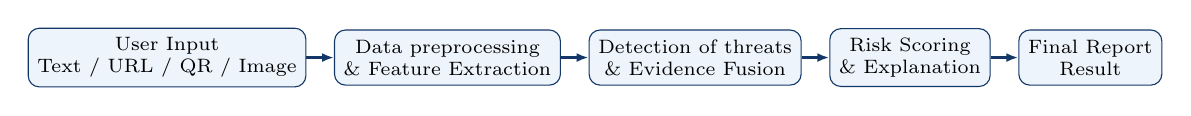
\begin{tikzpicture}[
node distance=3.5mm,
box/.style={
    rectangle,
    rounded corners,
    draw=GEUBlue,
    fill=GEULightBlue,
    minimum width=1.75cm,
    minimum height=7mm,
    align=center,
    font=\scriptsize
},
arrow/.style={
    -{Latex[length=1.5mm]},
    thick,
    draw=GEUBlue
}
]

\node[box] (a) {User Input\\Text / URL / QR / Image};
\node[box,right=of a] (b) {Data preprocessing\\\& Feature Extraction};
\node[box,right=of b] (c) {Detection of threats\\\& Evidence Fusion};
\node[box,right=of c] (d) {Risk Scoring\\\& Explanation};
\node[box,right=of d] (e) {Final Report\\Result};

\draw[arrow] (a)--(b);
\draw[arrow] (b)--(c);
\draw[arrow] (c)--(d);
\draw[arrow] (d)--(e);

\end{tikzpicture}
\end{center}
\vspace{5mm}

\begin{columns}[T,totalwidth=\textwidth]

\column{.48\textwidth}

\textbf{\color{GEUBlue}Major Components}

\begin{itemize}\itemsep2pt
    \item \placeholder{Multimodal Input \& Data preprocessing}
    \item \placeholder{Detection of threats \& Evidence Fusion}
    \item \placeholder{Risk Scoring \& Explainability}
\end{itemize}

\column{.48\textwidth}
\small

\textbf{\color{GEUBlue}Data / Control Flow}

\begin{itemize}\itemsep2pt
    \item \placeholder{An input(text, URL, QR code, or image) is uploaded by user.}
    \item \placeholder{ Features are extracted from each type of data and merged for analysis.}
    \item \placeholder{System predicts a risk score along with viable evidence to support the prediction.}
\end{itemize}

\end{columns}

\end{frame}
% 8
\begin{frame}{Technology Stack \& Methodology}

\begin{columns}[T,totalwidth=\textwidth]

\column{.48\textwidth}

\begin{block}{Technology Stack}
\begin{itemize}\itemsep2pt
\item Programming: \placeholder{Python / C / C++}
\item Database: \placeholder{MySQL / SQLite}
\item Tools / Framework: \placeholder{Scikit-learn, OpenCV, Streamlit}
\item IDE: \placeholder{VS Code / Jupyter Notebook}
\item Version Control: \placeholder{Git / GitHub}
\end{itemize}
\end{block}

\column{.48\textwidth}

\begin{block}{Development Methodology}
\begin{enumerate}\itemsep2pt
\item Analysis of requirements
\item Data Collection \& Data preprocessing
\item System Design
\item Model Development \& Integration
\item Testing \& Evaluation
\end{enumerate}
\end{block}

\end{columns}

\vfill

\begin{center}
\smallnote{The selected technologies support multimodal data processing,
ML based detection, rapid prototyping development.}
\end{center}

\end{frame}

% 9
\begin{frame}{Initial Progress \& Team Contribution}

\begin{columns}[T,totalwidth=\textwidth]

\column{.44\textwidth}

\textbf{\color{GEUBlue}Progress Achieved}

\begin{itemize}\itemsep3pt
\item \placeholder{Background and research study is  completed}
\item \placeholder{Problem statement is identified}
\item \placeholder{Multimodal system architecture is  prepared}
\item \placeholder{Initial detection modules is in production}
\item \placeholder{Dataset and data pre-processing pipeline is in production}
\end{itemize}

\column{.52\textwidth}

\textbf{\color{GEUBlue}Individual Contribution}

\vspace{2mm}

\scriptsize
\begin{tabularx}{\textwidth}{@{}p{1.8cm}p{2.0cm}X@{}}
\toprule
Member & Role & Contribution\\
\midrule
\placeholder{Shivansh} & \placeholder{Lead / ML} &
\placeholder{System architecture, ML pipeline designing}\\
\placeholder{Ashrey} & \placeholder{Developer} &
\placeholder{Research of detection modules and Data preprocessing}\\
\placeholder{Kangana} & \placeholder{Research / Testing} &
\placeholder{Background research and references, Dataset preparation }\\
\bottomrule
\end{tabularx}

\end{columns}

\end{frame}


% 10
\begin{frame}{Roadmap, Expected Outcomes \& References}

\scriptsize

\begin{columns}[T,totalwidth=\textwidth]

\column{.47\textwidth}

\textbf{\color{GEUBlue}Roadmap}

\begin{enumerate}\itemsep2pt \parskip0pt
\item Phase-I: Proposal of Problem Statement \& System Design
\item Phase-II: Data Collection, Model \& Pipeline Development
\item Phase-III: Integration, Training and Testing \& Final Implementation
\end{enumerate}

\vspace{2mm}

\textbf{\color{GEUBlue}Expected Outcomes}

\begin{itemize}\itemsep2pt \parskip0pt
\item A Multimodal prototype is made that can detect and classify scams according to the inputs by the user.
\item The prototype provides explainable risk scoring with supporting evidence  
\item To increase the scope for future scalability across
      new scam types, and detection models.
\end{itemize}

\column{.47\textwidth}

{\tiny
\textbf{\color{GEUBlue}References}

\vspace{1mm}

\begin{enumerate}\itemsep1pt \parskip0pt
\item CERT-In, ``Preventing Online Scams,'' 2024.
\item Sahingoz et al., ``Machine learning based phishing detection from URLs,''
      Expert Systems with Applications, 2019.
\item Trad and Chehab, ``Detecting Quishing Attacks with Machine Learning
      Techniques Through QR Code Analysis,'' 2025.
\item Sharevski et al., ``Gone Quishing: A Field Study of Phishing with
      Malicious QR Codes,'' 2022.
\item Anti-Phishing Working Group, ``Phishing Activity Trends Report,
      1st Quarter 2026,'' 2026.
\end{enumerate}
}

\vspace{4mm}

\begin{center}
\colorbox{GEUBlue}{%
\parbox{.78\textwidth}{%
\centering
\color{white}
\textbf{\small Thank You}\\[1mm]
\scriptsize Questions \& Suggestions
}}
\end{center}
\vspace{8mm}

\end{columns}

\end{frame}

\end{document}